% vim:ts=4:sw=4:expandtab
\documentclass[compress]{beamer}
\usepackage{fontspec}
\usepackage{listings}
\usepackage{tikz}
\usepackage[labelformat=empty]{caption}

\setmainfont{Trebuchet MS}
%\setmonofont{Inconsolata}
\setmonofont[SmallCapsFont={DejaVu Sans Mono}]{DejaVu Sans Mono}
\usetheme{default}

% white-ish on black-ish
\definecolor{myblack}{rgb}{1,1,1}
\definecolor{mywhite}{rgb}{0,0,0}

\setbeamertemplate{frametitle}{
    \color{mywhite}
    \vspace*{0.5cm}
    \hspace*{0.25cm}
    \textbf{\insertframetitle}
    \par
}

\setbeamercolor{background canvas}{bg=myblack}
\setbeamercolor{normal text}{fg=mywhite}

% Hide the navigation icons at the bottom of the page
\setbeamertemplate{navigation symbols}{}
% Slide numbers at the bottom of the page
\setbeamerfont{footline}{size=\fontsize{9}{11}\selectfont}
\setbeamertemplate{footline}[frame number]

\definecolor{darkblue}{rgb}{0,0,.6}
\definecolor{darkred}{rgb}{.6,0,0}
\definecolor{darkgreen}{rgb}{0,.6,0}
\definecolor{darkgray}{gray}{.3}
\definecolor{lightblue}{rgb}{0.97,0.99,1}
\definecolor{myblue}{rgb}{0.62,0.80,0.96}
\definecolor{mystring}{rgb}{0.74,0.76,0.41}
\lstdefinestyle{colors}{%
    keywordstyle={\bf\color{darkblue}},%
    commentstyle={\em\color{myblue}},%
    stringstyle={\color{mystring}},%
    emphstyle={\color{darkgray}}}
\lstset{language=C,style=colors,inputencoding=utf8,extendedchars=true,texcl,escapechar=\|,basicstyle=\small\ttfamily,keywordstyle=\bfseries,numbers=none,numberblanklines=false,showstringspaces=false,breaklines=true,numberstyle=\small\ttfamily,xleftmargin=\parindent,xrightmargin=1em,linewidth=0.98\linewidth}


%% Metadaten von Vortrag
%\newcommand{\datum}{2012-07-19}
%\newcommand{\autor}{Michael Stapelberg, Felix Bruckner, Pascal Krause}
%\newcommand{\vorlesung}{Parallele Rechnerarchitekturen}
%\newcommand{\semester}{SS2012}
%\newcommand{\ort}{Hochschule Mannheim}
%
\title{„kinectboard“ — Objekt-Tracking\\mit CUDA und Kinect}
\author{Michael Stapelberg, Felix Bruckner, Pascal Krause}
\institute{Fakultät für Informatik\\
           Hochschule Mannheim\\}
\date{2012-07-19}
%\beamertemplatetransparentcovereddynamic
%\setbeamerfont{note page}{size=\small}
%%\renewcommand{\>}{\rangle}
%%\newcommand{\<}{\langle} 
%%\usebeamercolor[fg]{[page number]}
%
%\setbeamertemplate{navigation symbols}{}
%%\setbeamertemplate{note page}{}
%
%%Zum Abschalten der kleinen Navigationsleiste am unteren Rand reicht folgende Zeile aus:
%%\beamertemplatenavigationsymbolsempty
%
%\setbeamersize{text margin left=0.2cm}
%\setbeamersize{text margin right=0.25cm}
%\setbeamersize{sidebar width right=0cm}
%\setbeamersize{sidebar width left=0cm}
%
%%Inhalt der Fußzeile festlegen
%\setbeamertemplate{footline}
%{
%\setbeamercolor{bgcolor}{fg=black,bg=white}
%\begin{beamercolorbox}{bgcolor}
%\hspace*{0.2cm}
%% \copyright 
%\autor\ -- \vorlesung\ -- \ort\ -- \semester
%\hfill
%%  \insertslidenavigationsymbol
%%  \insertframenavigationsymbol
%%  \insertsubsectionnavigationsymbol
%%  \insertsectionnavigationsymbol
%%  \insertdocnavigationsymbol
%%  \insertbackfindforwardnavigationsymbol
% \hfill\insertframenumber/\inserttotalframenumber
% \hspace*{0.2cm}
%\end{beamercolorbox}
%
%}
%
%%\newcommand{\markNote}[1]{	\textsuperscript{\tiny [#1]} }
%\newcommand{\markNote}[1]{	 }
%
%% Bei jeder Section ein Inhaltsverzeichnis ausgeben
% \AtBeginSection[]{
% \begin{frame}
% %\frametitle{Outline}
% \tableofcontents[current] % Nur die sections ausgeben
% \end{frame}
% }
%
%% Die Zeile definieren, die ganz oben ist und die Abschnitte enthält
%% Das sind die Maße wenn es die Folie "nächste Vorlesung gibt"
%% \setbeamertemplate{headline}
%% {%
%%   \begin{beamercolorbox}{section in head/foot}
%%     \vskip5pt\insertnavigation{12.4cm}\vskip5pt
%%   \end{beamercolorbox}%
%% }
%
%%\setbeamertemplate{headline}
%%{%
%%  \begin{beamercolorbox}{section in head/foot}
%%    \vskip5pt\insertnavigation{12.75cm}\vskip5pt
%%  \end{beamercolorbox}%
%%}
%
%\begin{document}
%
% Deckblatt generieren
\begin{document}
\begin{frame}
\titlepage
\end{frame}

% Inhaltsverzeichnis am Anfang des Dokuments
\begin{frame}
  %\frametitle{Heute}
  %\tableofcontents[hideallsubsections]  % Nur die sections ausgeben
  \tableofcontents                       % sections und subsections ausgeben
\end{frame}

%Allgemeines zu S3
\section{Allgemeines}
\subsection{Unser Projekt}
\begin{frame}
\frametitle{Projektidee: Objekttracking}

Jede einigermaßen ebene Fläche soll als Whiteboard dienen können.

\begin{itemize}
	\item Schwierigkeiten
	\begin{itemize}
		\item Pure Farberkennung zu viele false-positives
		\item Qualität des Tiefenbildes zu schlecht
	\end{itemize}
	\item Lösungsansatz
		\begin{itemize}
		\item Aufbereitung der Daten durch Anwenden von Filtern
	\end{itemize}
\end{itemize}
\end{frame}

\subsection{Vorgehen}

\begin{frame}
\frametitle{Vorgehen}

\begin{itemize}
	\item Suchen eines open-source SDKs
	\item Erforschen der Kinect
	\item Suchen nach Problemlösungen
	\item Validieren der Lösungen (CPU)
	\item Portieren der Lösungen auf GPU
	\begin{itemize}
		\item Programmaufbau an CUDA anpassen 
		\item Algorithmen für CUDA optimieren
	\end{itemize}
	
\end{itemize}
\end{frame}

\subsection{Hardware}

\begin{frame}
\frametitle{Kinect}

\hspace*{1.8cm}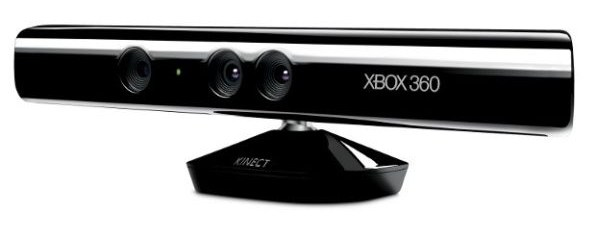
\includegraphics[width=8.5cm]{kin.jpg}

\begin{itemize}
	\item Sensoren
	\begin{itemize}
		\item 640x480 \@ 30Hz Farbbild (RGB)
		\item 640x480 \@ 30Hz Tiefenbild
	\end{itemize}
    \item Versetzte Kameras
	\item Genauigkeit
	\begin{itemize}
		\item Genauigkeit ab 50cm ca. 1,5mm
		\item Genauigkeit ab 5m ca. 5cm
	\end{itemize}
\end{itemize}
\end{frame}

\begin{frame}
\frametitle{Grafikkarte}

\hspace*{1.8cm}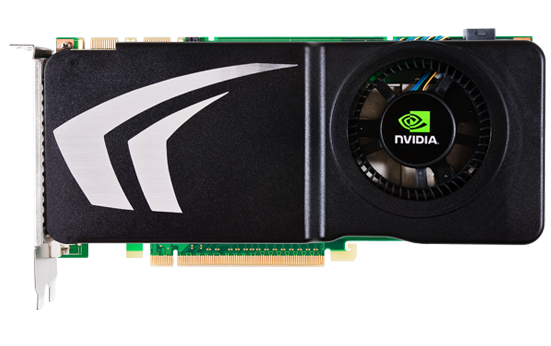
\includegraphics[width=8.5cm]{gts250.png}

\begin{itemize}
	\item nVidia GeForce GTS 250
	\item 16 Multiprozessoren mit je 8 CUDA-Cores
    \item CUDA Compute Capability 1.1
	\item 1024 MB Device-Memory	
\end{itemize}
\end{frame}

\begin{frame}
\frametitle{Handschuh}

\hspace*{2.5cm}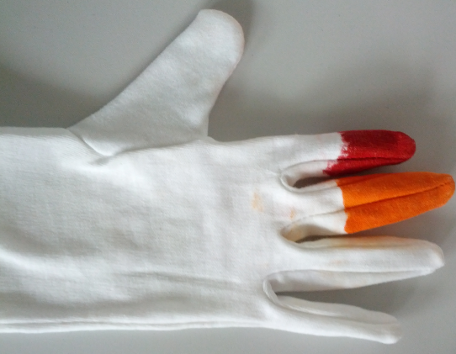
\includegraphics[width=7cm]{handschuh.png}

\begin{itemize}
	\item 100\% Baumwolle
	\item Hoher Tragekomfort
	\item Farbe: Orange
\end{itemize}
\end{frame}

\section{Algorithmen}

\subsection{Median-Filter}
\begin{frame}
\frametitle{Median-Filter}
\begin{itemize}
	\item Arbeitet auf dem Tiefenbild
	\item Filtert das Rauschen aus dem Tiefenbild heraus
\end{itemize}
\vspace*{1cm}

\begin{center}
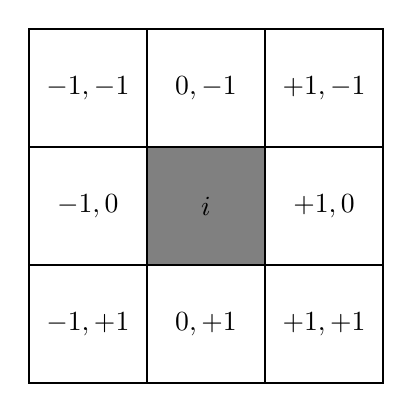
\begin{tikzpicture}[every node/.style={draw,outer sep=0pt,thick,minimum width=1.5cm,minimum height=1.5cm}]
    \node[fill=gray] (i) {$i$};
    \node (im1) at (i.west) [anchor=east] {$-1, 0$};
    \node (ip1) at (i.east) [anchor=west] {$+1, 0$};

    % obere Reihe
    \node (im1m1) at (im1.north) [anchor=south] {$-1, -1$};
    \node (im1m0) at (i.north) [anchor=south] {$0, -1$};
    \node (im1p1) at (ip1.north) [anchor=south] {$+1, -1$};

    % untere Reihe
    \node (ip1m1) at (im1.south) [anchor=north] {$-1, +1$};
    \node (ip1m0) at (i.south) [anchor=north] {$0, +1$};
    \node (ip1p1) at (ip1.south) [anchor=north] {$+1, +1$};
\end{tikzpicture}
\end{center}
\end{frame}

\begin{frame}
\frametitle{Median-Filter}
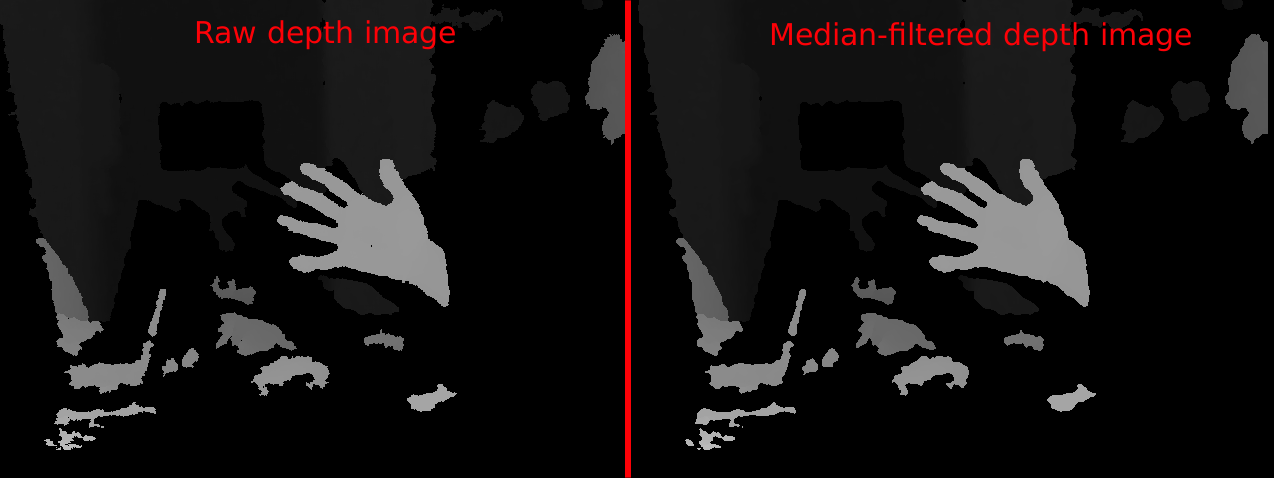
\includegraphics[width=\textwidth]{filter1.png}
\end{frame}

\subsection{Kalibrierung}
\begin{frame}
\frametitle{Kalibrierung}
\begin{itemize}
	\item Es kann auf neuen Hintergrund kalibriert werden
	\item Arbeitet auf dem Tiefenbild
	\item Filtert alle sich nicht bewegenden Punkte aus dem Tiefenbild.
\end{itemize}
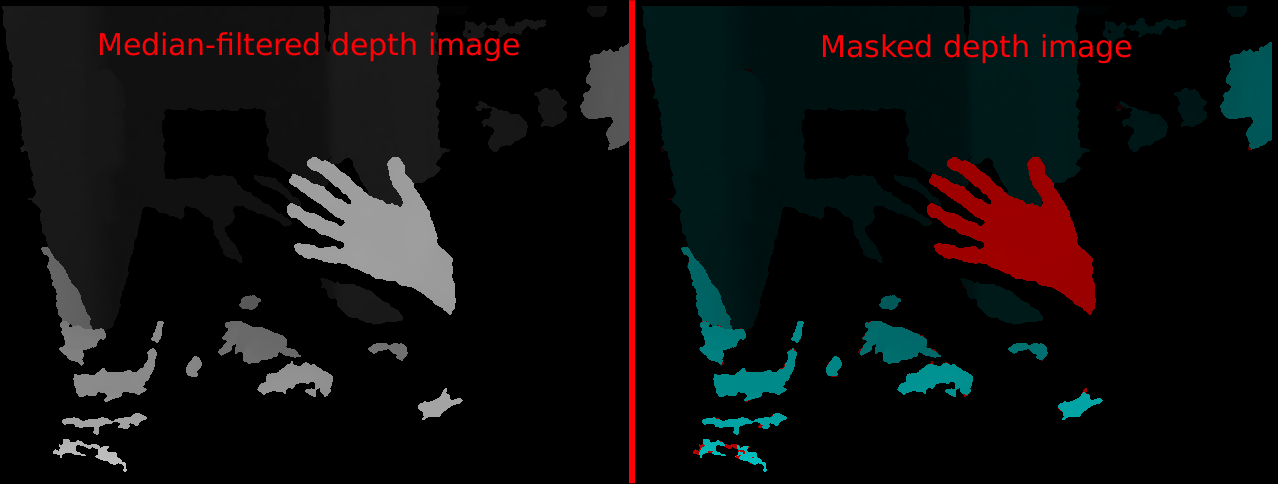
\includegraphics[width=\textwidth]{filter2.png}
\end{frame}

\subsection{Gloweffekt}
\begin{frame}
\frametitle{Gloweffekt}
\begin{itemize}
	\item Arbeitet auf dem Tiefenbild
	\item Expandiert alle anzuzeigenden Punkte im Tiefenbild, anhand eines einstellbaren Radius
\end{itemize}
\vspace*{0.5cm}
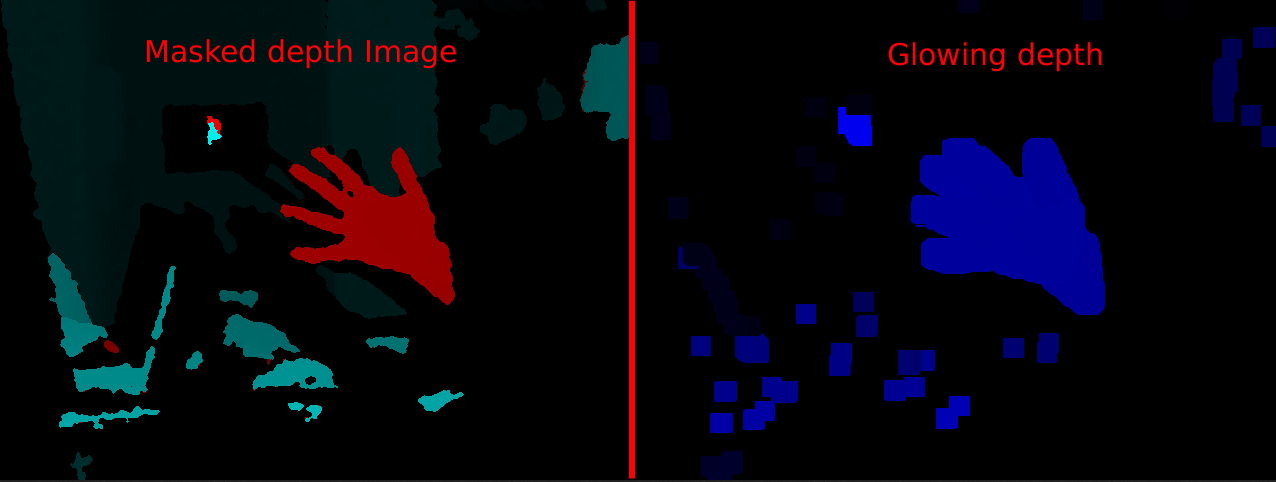
\includegraphics[width=\textwidth]{filter3.png}
\end{frame}

\subsection{RGB-Bild maskieren}
\begin{frame}
\frametitle{RGB-Bild maskieren}
\begin{itemize}
	\item Arbeitet auf dem RGB-Bild
	\item Rechnet das Tiefenbild auf das RGB-Bild um, und maskiert alle relevanten Pixel
\end{itemize}

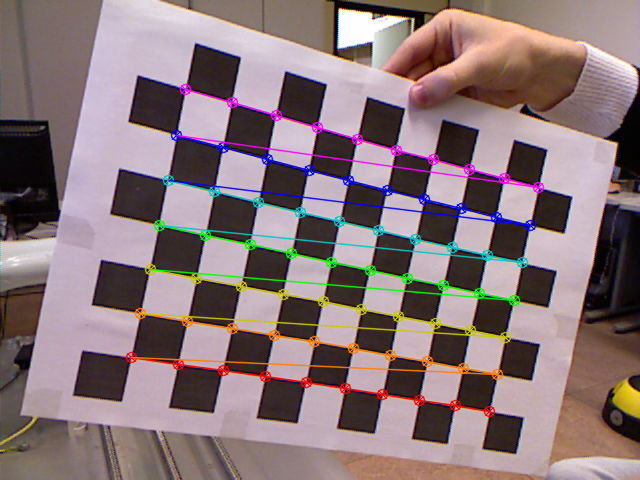
\includegraphics[width=0.5\textwidth]{trans.png}
\end{frame}

\subsection{Referenz-Farbe}
\begin{frame}
\frametitle{Referenz-Farbe}
\begin{itemize}
	\item Arbeitet auf dem RGB-Bild
	\item Zeigt nur noch die Pixel auf dem RGB-Bild an, welche farblich ähnlich genug zur Referenzfarbe sind
\end{itemize}

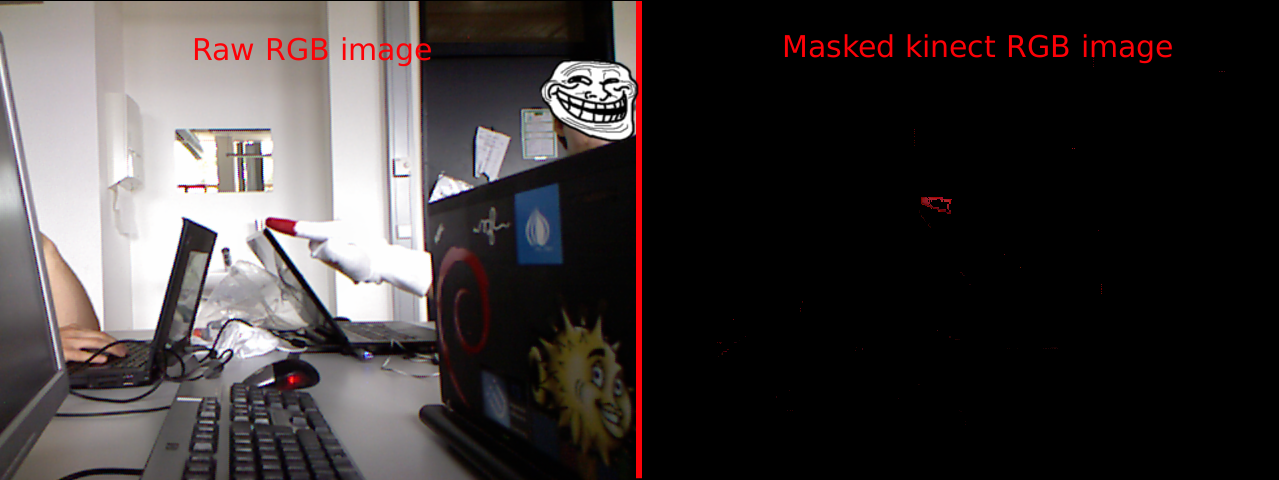
\includegraphics[width=\textwidth]{filter4.png}
\end{frame}

\begin{frame}{Median-Filter: Überblick}
    \newcounter{overviewstep}
    \begin{list}{\arabic{overviewstep}.}{\usecounter{overviewstep}\itemsep=1em}
        \item Host: Bilddaten auf die Grafikkarte kopieren, Kernel starten
        \item Index berechnen, (umliegende) Pixel-Werte lesen
        \item Median-Filter anwenden
        \item Pixel-Wert umwandeln in RGB-Wert
        \item Ausgabe-Pixel schreiben
        \item Host: Bild anzeigen
    \end{list}
\end{frame}

\begin{frame}[fragile]{Wert lesen und umrechnen (readpixel0)}
\begin{lstlisting}
__global__ void median(uint16_t *depth,
    uint8_t *table, uint8_t *output)
{
  int x = blockIdx.x * blockDim.x + threadIdx.x;
  int y = blockIdx.y * blockDim.y + threadIdx.y;
  int i = (y * 640) + x;

  // Pixel in RGB wandeln
  int conv = table[depth[i]];

  // Makro, welches output[i], output[i+1] und output[i+2] setzt.
  pushrgb(output, i, conv);
}
\end{lstlisting}
\end{frame}

\begin{frame}[fragile]{Wert lesen und umrechnen (readpixel0)}
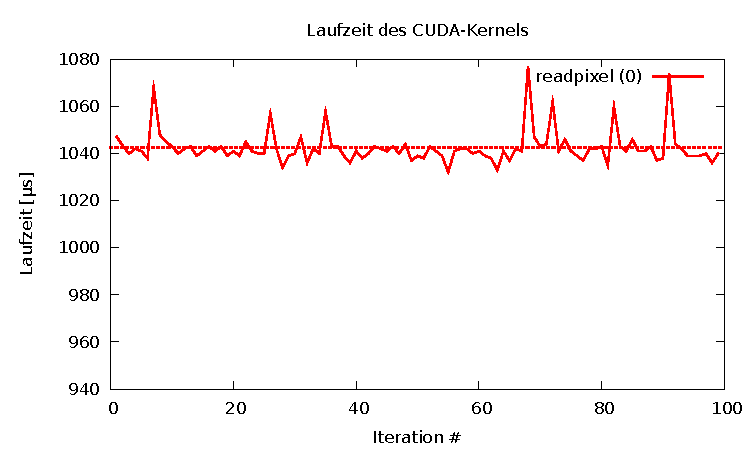
\includegraphics[width=\textwidth]{readpixel0.pdf}
\end{frame}

\begin{frame}[fragile]{Wert lesen und umrechnen (readpixel0/1)}
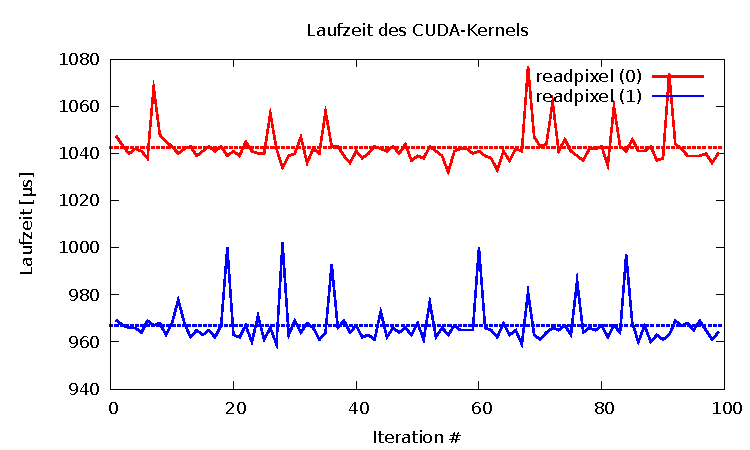
\includegraphics[width=\textwidth]{readpixel01.pdf}
\end{frame}

\begin{frame}[fragile]{Wert lesen und umrechnen (readpixel1)}
\begin{lstlisting}
texture<uint16_t, 2> depthT;
texture<uint8_t, 2> tableT;

__global__ void median(uint8_t *output) {
  // x, y, i wie zuvor
  int c = tex2D(tableT, tex2D(depthT, x, y), 1);
  pushrgb(output, i, c);
}

// memcpy table und depth

cudaChannelFormatDesc desc = cudaCreateChannelDesc<uint16_t>();
cudaBindTexture2D(NULL, &depthT, depth, &desc, 640, 480, 640 * sizeof(uint16_t));
desc = cudaCreateChannelDesc<uint8_t>();
cudaBindTexture2D(NULL, &tableT, table, &desc, 2048, 1, 2048 * sizeof(uint8_t));
\end{lstlisting}
\end{frame}

\begin{frame}[fragile]{Wert lesen und umrechnen (readpixel0/1/2)}
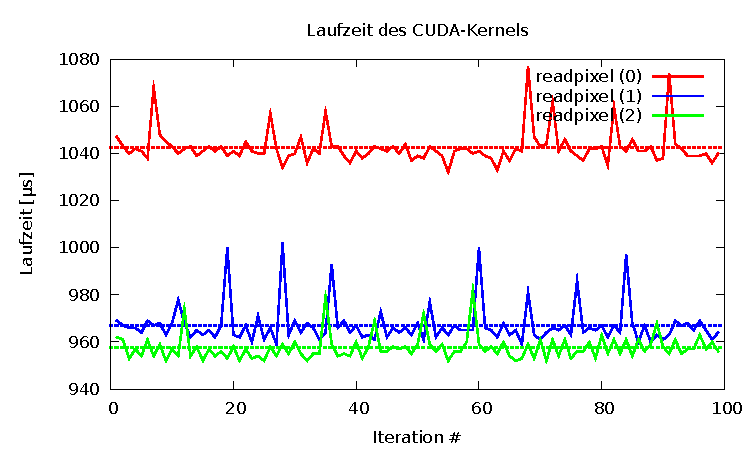
\includegraphics[width=\textwidth]{readpixel12.pdf}
\end{frame}


\begin{frame}[fragile]{Wert lesen und umrechnen (readpixel2)}
\begin{lstlisting}
texture<uint16_t, 2> depthT;
texture<uint8_t, 2> tableT;

__global__ void median(uint8_t *output) {
  // x, y, i wie zuvor
  int d = tex2D(depthT, x, y);
  int c = (float)(2048 * 256) / (d - 2048);

  pushrgb(output, i, c);
}

// memcpy table und depth
// cudaBindTexture2D wie zuvor
\end{lstlisting}
\end{frame}

\begin{frame}[fragile]{Median-Filter (median3)}
\begin{lstlisting}
__global__ void median(uint8_t *output) {
  // x, y, i wie zuvor
  int neigh[25], ic, ir, ni = 0;
  for (ic  = (x - (5 / 2));
       ic <= (x + (5 / 2));
       ic++) {
    for (ir  = (y - (5 / 2));
         ir <= (y + (5 / 2));
         ir++) {
      neigh[ni++] = tex2D(depthT, ic, ir);
    }
  }

  // quick\_select aus "Numerical recipes in C"
  int c = (float)(2048 * 256) / (quick_select(neigh, 25) - 2048);
  pushrgb(output, i, c);
}
\end{lstlisting}
\end{frame}

\begin{frame}[fragile]{Median-Filter (median3)}
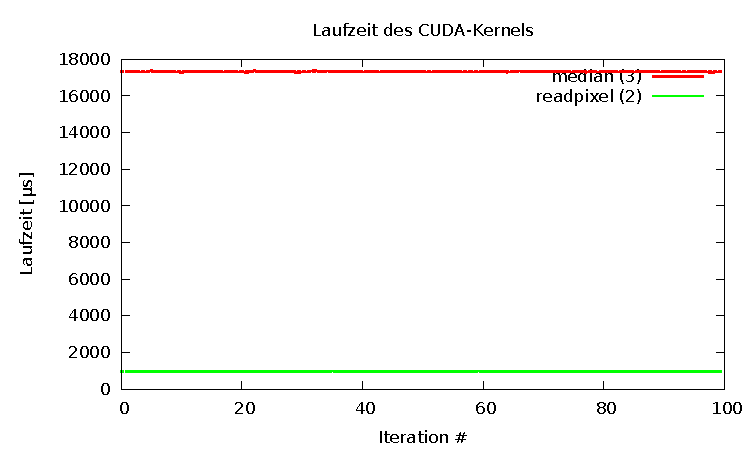
\includegraphics[width=\textwidth]{median3.pdf}
\end{frame}

\begin{frame}[fragile]{Median-Filter (median3/5)}
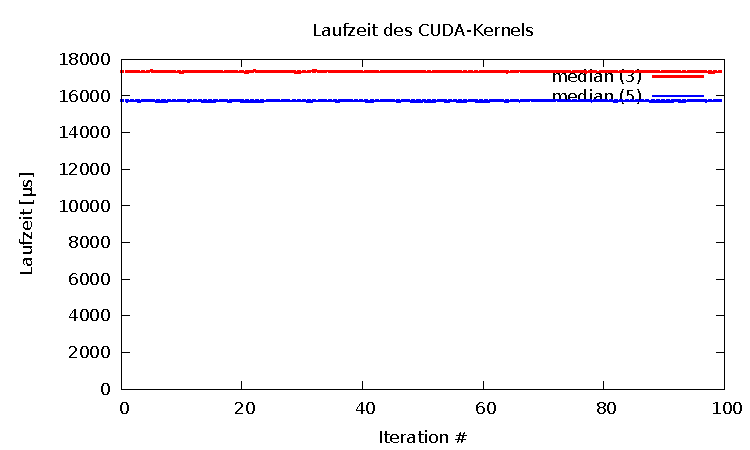
\includegraphics[width=\textwidth]{median35.pdf}
\end{frame}


\begin{frame}[fragile]{Median-Filter (median5)}
\begin{lstlisting}
__global__ void median(uint8_t *output) {
  __shared__ float smem[BLOCK_X][BLOCK_Y];
  smem[threadIdx.x][threadIdx.y] = tex2D(depthT, x, y);
  __syncthreads();

  int neigh[25], ic, ir, ni = 0;
  for (ic  = (threadIdx.x - (5 / 2));
       ic <= (threadIdx.x + (5 / 2));
       ic++) {
    for (ir  = (threadIdx.y - (5 / 2));
         ir <= (threadIdx.y + (5 / 2));
         ir++) {
      neigh[ni++] = smem[ic][ir];
    }
  }

  // quick\_select wie zuvor
}
\end{lstlisting}
\end{frame}

\begin{frame}[fragile]{Median-Filter (median5/8)}
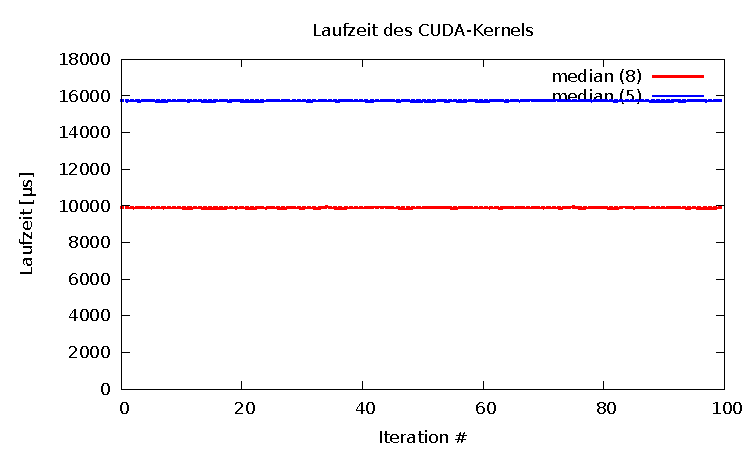
\includegraphics[width=\textwidth]{median58.pdf}
\end{frame}

\begin{frame}[fragile]{Median-Filter (median8)}
\begin{lstlisting}
__global__ void median(uint8_t *output) {
    int ic, ir, ni = 0;
    float neigh[9], ma, mi;
    for (ic = (x - 1); ic <= (x + 1); ic++) {
      for (ir = (y - 1); ir <= (y + 1); ir++) {
        neigh[ni++] = tex2D(depthT, ic, ir);
      }
    }
    for (int i = 0; i < 8; i++) {
      for (int j = 0; j < (8-i); j++) {
        ma = fmaxf(neigh[j], neigh[j+1]);
        mi = fminf(neigh[j], neigh[j+1]);
        neigh[j] = mi;
        neigh[j+1] = ma;
      }
    }
    int c = (float)(2048 * 256) / (neigh[9/2] - 2048.0);
}
\end{lstlisting}
\end{frame}


\begin{frame}[fragile]{Median-Filter (median8/8u)}
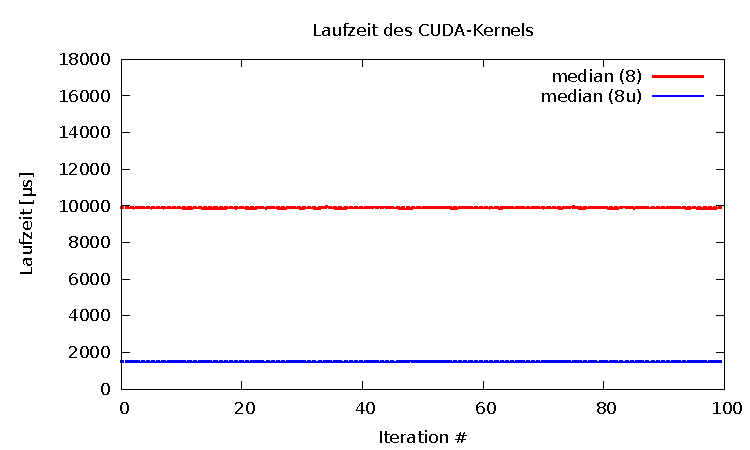
\includegraphics[width=\textwidth]{median88u.pdf}
\end{frame}

\begin{frame}[fragile]{Median-Filter, PTX (median8)}
\lstset{basicstyle=\tiny\ttfamily}
\begin{lstlisting}
$Lt_0_5634:
 //<loop> Loop body line 89, nesting depth: 1, iterations: 8
    mov.u32     %r58, 0;
    setp.le.s32     %p1, %r57, %r58;
    @%p1 bra    $Lt_0_5890;
    mov.s32     %r59, %r57;
    mov.u64     %rd1, __cuda___cuda_local_var_19377_11_non_const_nneighbors_1624;
    mov.s32     %r60, 0;
    mov.s32     %r61, %r59;
$Lt_0_6402:
 //<loop> Loop body line 89, nesting depth: 2, estimated iterations: unknown
    .loc    16  96  0
    ld.local.f32    %f70, [%rd1+0];
    ld.local.f32    %f71, [%rd1+4];
    max.f32     %f72, %f70, %f71;
    .loc    16  98  0
    min.f32     %f73, %f70, %f71;
    st.local.f32    [%rd1+0], %f73;
    .loc    16  99  0
    st.local.f32    [%rd1+4], %f72;
    add.s32     %r60, %r60, 1;
    add.u64     %rd1, %rd1, 4;
    setp.ne.s32     %p2, %r57, %r60;
    @%p2 bra    $Lt_0_6402;
\end{lstlisting}
\end{frame}

\begin{frame}[fragile]{Median-Filter (median8)}
\lstset{basicstyle=\small\ttfamily}
\begin{lstlisting}
__global__ void median(uint8_t *output) {
    int ic, ir, ni = 0;
    float neigh[9], ma, mi;
    for (ic = (x - 1); ic <= (x + 1); ic++) {
      for (ir = (y - 1); ir <= (y + 1); ir++) {
        neigh[ni++] = tex2D(depthT, ic, ir);
      }
    }
    for (int i = 0; i < 8; i++) {
      for (int j = 0; j < 8; j++) {
        ma = fmaxf(neigh[j], neigh[j+1]);
        mi = fminf(neigh[j], neigh[j+1]);
        neigh[j] = mi;
        neigh[j+1] = ma;
      }
    }
    int c = (float)(2048 * 256) / (neigh[9/2] - 2048.0);
}
\end{lstlisting}
\end{frame}

% Man kann den obigen Algorithmus noch anders aufschreiben (unrolled), dann
% wird er nochmal ca. 100 usec schneller, aber Lesbarkeit leidet.

\begin{frame}[fragile]{Fazit}
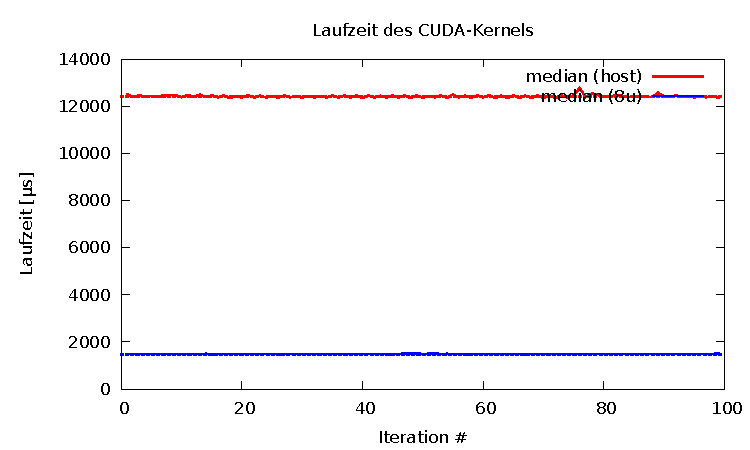
\includegraphics[width=\textwidth]{medianhost.pdf}\\
\begin{center}
Speedup durch CUDA: $\approx 12x$
\end{center}
\end{frame}
\section{Hardware-Rendering}

\begin{frame}
\frametitle{Portierung auf GPU}
\begin{itemize}
\item Ausgangssituation (Proof of concept, CPU)
	\begin{itemize}
		\item SDL Surface
		\item Softwarerendering
		\item 3 FPS bei Einschalten der Filter
	\end{itemize}
\item Ziel (GPU)
	\begin{itemize}
		\item Bilder von Host auf Grafikkarte kopieren
		\item Bilder auf Grafikkarte berechnen
		\item Bilder von Grafikkarte auf Host kopieren
		\item extrem langsam (memcpy-overhead)
	\end{itemize}
\end{itemize}
\end{frame}

\subsection{Minimierung der Datentransfers}
\begin{frame}
\frametitle{Minimierung der Datentransfers}
\begin{itemize}
\item Alle Bilder in einen Block
\item Weniger Memcopys
\item Immernoch zu langsam (5fps)
\item Kosten für ein Memcopy 7ms
\item Maximale Durchlaufdauer 30ms
\end{itemize}
\end{frame}

\subsection{GPU-Buffer mit OpenGL direkt rendern}
\begin{frame}[fragile]
\frametitle{GPU-Buffer mit OpenGL direkt rendern}
\begin{itemize}
\item Hardwarerendering mit OpenGL
\item OpenGL Pixel Buffer Objects (PBOs)
\item Nur noch Kopieren der Input-Bilder erforderlich
\end{itemize}
\begin{lstlisting}
cutilSafeCall(cudaGLMapBufferObject((void**)&gpu_raw_depth_output, rawDepthBufferID));
// Process data on GPU
cutilSafeCall(cudaGLUnmapBufferObject(rawDepthBufferID));

glBindBuffer(GL_PIXEL_UNPACK_BUFFER, img_->bufferID);
glBindTexture(GL_TEXTURE_2D, img_->textureID);
glTexSubImage2D(GL_TEXTURE_2D, 0, 0, 0, 640, 480, GL_RGBA, GL_UNSIGNED_BYTE, NULL);
// Setup texture position
\end{lstlisting}
\end{frame}

\subsection{Flüssige Darstellung}
\begin{frame}
\frametitle{Flüssige Darstellung}
\begin{itemize}
\item Doublebuffering verhindert flackern
\item BufferObjekt besteht aus front \& back
\item Bufferwechsel bei Pixelveränderung
\item VSync
\end{itemize}
\hspace*{4cm}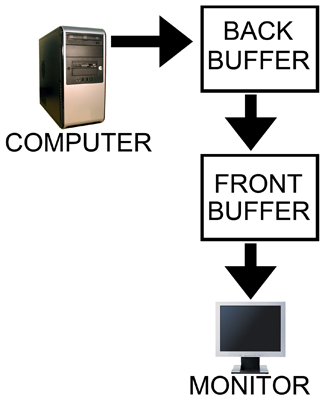
\includegraphics[width=3cm]{double.png}
\end{frame}

\subsection{GUI}
\begin{frame}
\frametitle{GUI}
\begin{itemize}
\item Alte SDL-GUI keine OpenGL-Unterstützung
\item Experimentelle Bestimmung der Schwellwerte etc.
\item Anzeige von Zustand und Parametern
\item OpenGL-GUI basiert auf Awesomium (Browser-Engine)
\end{itemize}
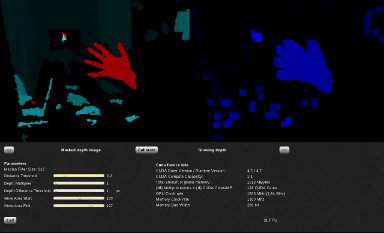
\includegraphics[width=\textwidth]{gui.png}
\end{frame}

\section{Live-Demo}
\begin{frame}{Live-Demo}
\Huge
\centerline{Live-Demo}
\end{frame}

\section{Ausblick}

\begin{frame}
\frametitle{Ausblick}
\begin{itemize}
	\item Bewegung interpolieren
	\item Extremitäten statt Pixel
	\item Visuell bedienbare GUI
	\begin{itemize}
		\item Buttons
		\item Gesten
	\end{itemize}
	\item Ausführlichere Dokumentation
	\item Plattformabhängigkeit minimieren
\end{itemize}
\end{frame}

\begin{frame}
\Huge
\centerline{Vielen Dank}
\centerline{für Ihre Aufmerksamkeit}
\end{frame}



\end{document}
